\documentclass[a4paper,twoside]{article}
\usepackage{blindtext}
\usepackage{geometry}

% Chinese support
\usepackage[UTF8, scheme = plain]{ctex}

% Page margin layout
\geometry{left=2.3cm,right=2cm,top=2.5cm,bottom=2.0cm}

\usepackage{listings}
\usepackage{xcolor}
\usepackage{geometry}
\usepackage{amsmath}
\usepackage{float}
\usepackage{hyperref}

\usepackage{graphics}
\usepackage{graphicx}
\usepackage{subfigure}
\usepackage{epsfig}
\usepackage{float}

% \usepackage{algorithm}
\usepackage[noend]{algpseudocode}

\usepackage{booktabs}
\usepackage{threeparttable}
\usepackage{longtable}
\usepackage{listings}
\usepackage{tikz}
\usepackage{multicol}

% cite package, to clean up citations in the main text. Do not remove.
\usepackage{cite}

\usepackage{color,xcolor}

%% The amssymb package provides various useful mathematical symbols
\usepackage{amssymb}
%% The amsthm package provides extended theorem environments
\usepackage{amsthm}
\usepackage{amsfonts}
\usepackage{enumerate}
\usepackage{enumitem}
\usepackage{listings}

\usepackage[ruled,linesnumbered]{algorithm2e}
\usepackage{indentfirst}
\setlength{\parindent}{2em} % Make two letter space in the first paragraph
\usepackage{setspace}
\linespread{1.5} % Line spacing setting
\usepackage{siunitx}
\setlength{\parskip}{0.5em} % Paragraph spacing setting

\renewcommand{\figurename}{图}
\renewcommand{\lstlistingname}{代码} 
\renewcommand{\tablename}{表格}
\renewcommand{\contentsname}{目录}

\graphicspath{ {images/} }
\newcommand{ \upcitep}[1]{\textsuperscript{\textsuperscript{\citep{#1} } }} % 设置上标显示参考文献编号的命令
%%%%%%%%%%%%%
\newcommand{\StudentNumber}{}  % Fill your student number here
\newcommand{\StudentName}{刘本宸、黄子扬}  % Replace your name here
\newcommand{\PaperTitle}{DNA计算理论的历史和前沿发展}  % Change your paper title here
\newcommand{\PaperType}{非经典计算课程报告} % Replace the type of your report here
\newcommand{\Date}{2023年5月10日}
\newcommand{\College}{信息学院}
\newcommand{\CourseName}{非经典计算}
%%%%%%%%%%%%%

%% Page header and footer setting
\usepackage{fancyhdr}
\usepackage{lastpage}
\pagestyle{fancy}
\fancyhf{}
% This requires the document to be twoside
\fancyhead[LO]{\texttt{\StudentName }}
\fancyhead[LE]{\texttt{\StudentNumber}}
\fancyhead[C]{\texttt{\PaperTitle }}
\fancyhead[R]{\texttt{第{\thepage} 页,共 \pageref*{LastPage} 页}}

\title{\PaperTitle}
\author{\StudentName}
\date{\Date}


\lstset{
	basicstyle          =   \sffamily,          % 基本代码风格
	keywordstyle        =   \bfseries,          % 关键字风格
	commentstyle        =   \rmfamily\itshape,  % 注释的风格,斜体
	stringstyle         =   \ttfamily,  % 字符串风格
	flexiblecolumns,                % 别问为什么,加上这个
	numbers             =   left,   % 行号的位置在左边
	showspaces          =   false,  % 是否显示空格,显示了有点乱,所以不现实了
	numberstyle         =   \zihao{-5}\ttfamily,    % 行号的样式,小五号,tt等宽字体
	showstringspaces    =   false,
	captionpos          =   t,      % 这段代码的名字所呈现的位置,t指的是top上面
	frame               =   lrtb,   % 显示边框
}

\lstdefinestyle{PythonStyle}{
	language        =   Python, % 语言选Python
	basicstyle      =   \zihao{-5}\ttfamily,
	numberstyle     =   \zihao{-5}\ttfamily,
	keywordstyle    =   \color{blue},
	keywordstyle    =   [2] \color{teal},
	stringstyle     =   \color{magenta},
	commentstyle    =   \color{red}\ttfamily,
	breaklines      =   true,   % 自动换行,建议不要写太长的行
	columns         =   fixed,  % 如果不加这一句,字间距就不固定,很丑,必须加
	basewidth       =   0.5em,
}

\lstdefinestyle{CppStyle}{
	language        =   c++,
	basicstyle      =   \zihao{-5}\ttfamily,
	numberstyle     =   \zihao{-5}\ttfamily,
	keywordstyle    =   \color{blue},
	keywordstyle    =   [2] \color{teal},
	stringstyle     =   \color{magenta},
	commentstyle    =   \color{red}\ttfamily,
	breaklines      =   true,   % 自动换行,建议不要写太长的行
	columns         =   fixed,  % 如果不加这一句,字间距就不固定,很丑,必须加
	basewidth       =   0.5em,
}

\algnewcommand\algorithmicinput{\textbf{Input:}}
\algnewcommand\algorithmicoutput{\textbf{Output:}}
\algnewcommand\Input{\item[\algorithmicinput]}%
\algnewcommand\Output{\item[\algorithmicoutput]}%
\renewcommand{\abstractname}{\textbf{\zihao{3}摘\quad 要}}
\usetikzlibrary{positioning, shapes.geometric}


\begin{document}

\makeatletter % change default title style
\renewcommand*\maketitle{%
	\begin{center}
		\bfseries  % title 
		{\LARGE \@title \par}  % LARGE typesetting
		\vskip 1em  %  margin 1em
			{\global\let\author\@empty}  % no author information
			{\global\let\date\@empty}  % no date
		\thispagestyle{empty}   %  empty page style
	\end{center}%
	\setcounter{footnote}{0}%
}
\makeatother

\thispagestyle{empty}

\vspace*{1cm}

\begin{figure}[h]
	\centering
	
\includegraphics[width=4.0cm]{logo.png}
\end{figure}

\vspace*{1cm}

\begin{center}
	\Huge{\textbf{\PaperType}}

	\Large{\PaperTitle}
\end{center}

\begin{table}[h]
	\centering
	\begin{Large}
		\renewcommand{\arraystretch}{1.5}
		\begin{tabular}{p{3cm} p{5cm}<{\centering}}
			姓 \quad 名 & \StudentName                         \\
			\hline
			学 \quad 号 & 22920202200764 \quad  22920202202789 \\
			\hline
			日 \quad 期 & \Date                                \\
			\hline
			学 \quad 院 & \College                             \\
			\hline
			课程名称    & \CourseName                          \\
			\hline
			教 \quad 师 & 曾华琳                               \\
		\end{tabular}
	\end{Large}
\end{table}

\newpage

\begin{abstract}
	本文主要梳理了DNA计算发展四十年以来一些关键性的进展,然后用了两个例子来讲述近几年来
	DNA计算最新的进展。我们先引入了DNA计算的最早的概念,Adleman的实验开辟了DNA计算这一领域的先河。
	后面我们讲到了使用DNA分子来模拟逻辑运算,这一研究发明了DNA逻辑门。DNA逻辑门的发明推动了后面DNA自动机以及
	DNA卷积神经网络的研究。近些年来,有些研究者使用DNA-自动机来模拟与人们进行井字棋对弈,也有一些研究者在使用DNA
	来模拟现有最火的卷积神经网络模型。这些研究在本文中都有所涉猎和讲解。


	\noindent{\textbf{关键词:}DNA计算,DNA逻辑门,DNA自动机,DNA卷积神经网络}
\end{abstract}
\newpage

\tableofcontents
\newpage


\section{DNA计算理论的提出}
\subsection{实验步骤}
Adleman\cite{ref1}提出的碱基互补配对原则是指在DNA分子中,腺嘌呤(A)始终与胸腺嘧啶(T)形成互补配对,
而鸟嘌呤(G)始终与胞嘧啶(C)形成互补配对。而这样的配对原则使得DNA计算成为可能。
在问题计算中,Adleman想要利用这个原理来解决一个指定的NP完全问题,即哈密顿路径问题\ref{ham}。

他先是构造一个DNA分子池,并且使用DNA分子编码问题的解空间,并利用碱基互补配对原则进行问题计算。
具体来说,Adleman将问题的每个可能解表示为一个DNA序列,并将这些DNA序列混合在一起形成一个DNA分子池。
然后,他将问题的输入表示为一个DNA序列,并将其与DNA分子池中的DNA序列进行杂交反应,以诱导形成包含问题的可能解的DNA序列的部分匹配。
这部分匹配主要是用到了DNA的碱基互补原则。比如在文中Aldeman提到了如何用碱基序列对一个图中的“顶点”和“边”进行建模和转化\ref{dna-encoding}。
\begin{itemize}
	\item 顶点 \quad
	      我们记$O_i$为顶点$i$,用一个有20个碱基长度的序列表示
	\item 边 \quad
	      我们记$O_{i \rightarrow j}$为顶点$i$到顶点$j$的一条边,用一个有20个碱基长度的序列表示
	      $O_{i \rightarrow j}$的前半段是$O_i$最后十个碱基结合而成的,
	      $O_{i \rightarrow j}$的后半段是$O_j$前十个碱基结合而成的。
	\item 顶点的补
	      我们记$\bar{O_i}$为顶点$O_i$的补。从上面边和顶点的定义我们可以通过两个边来组成一个顶点的补,
	      然后通过碱基的互补配对原则生成中间顶点
\end{itemize}

\begin{figure}[htbp]
	\centering
	\subfigure[哈密尔顿回路问题]{
		\begin{minipage}[t]{0.4\linewidth}
			\centering
			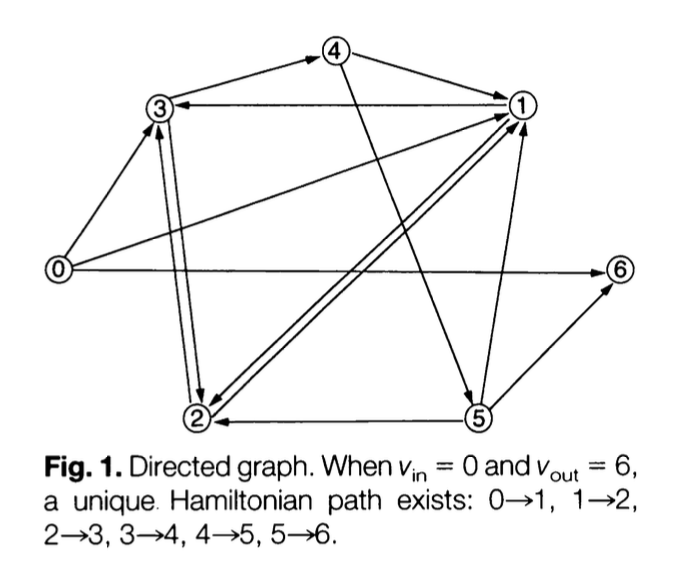
\includegraphics[width=6cm]{images/aldeman-article1.png}
			\label{ham}
		\end{minipage}
	}
	\subfigure[碱基的编码系统]{
		\begin{minipage}[t]{0.4\linewidth}
			\centering
			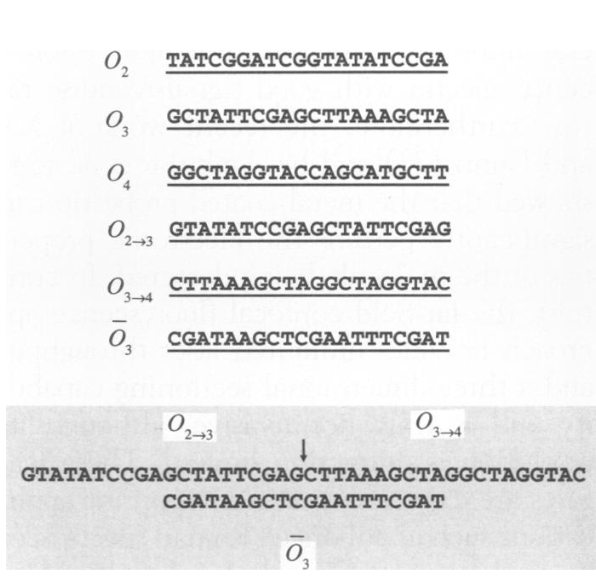
\includegraphics[width=6cm]{images/aldeman-article2.png}
			\label{dna-encoding}
		\end{minipage}
	}
	\qquad
	\subfigure[DNA计算后的电泳结果]{
		\begin{minipage}[t]{1\linewidth}
			\centering
			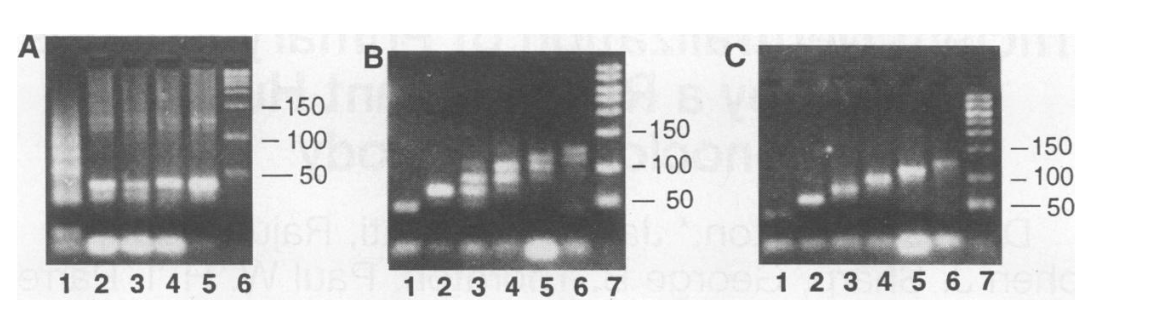
\includegraphics[width = 0.9\linewidth]{images/aldeman-article3.png}
			\label{gel-electro}
		\end{minipage}
	}
	\caption{Aldeman的实验}
\end{figure}
\newpage
接下来,Adleman使用PCR技术扩增这些匹配DNA序列,从而增加它们的数量。
最后,他对扩增后的DNA序列进行测序分析(电泳),以确定哪些DNA序列表示问题的解\ref{gel-electro}。
在这个电泳的结果图可以先看右轴,指示的是用于计算的DNA的碱基序列长度。
这个实验的最终产物在最右图中可以看到,一条条亮线代表了这个哈密尔顿回路的顶点遍历顺序。

\subsection{算法实现}
\begin{algorithm}[ht]
	\SetAlgoLined
	\caption{Adleman 的哈密尔顿图求解算法}\label{algorithm}
	\KwData{$S  \leftarrow$ 随机生成 $N$ 条碱基代表图的通路,$n  \leftarrow$图的顶点个数}
	\KwResult{$S^{\ast}$ 如果为空即输出 $No$,否则输出$Yes$}
	initialization\;
	$S_1  \leftarrow$ Select path begin with $v_0$ and end with$v_6$ from $S$ \;
	$S_2  \leftarrow$ Keep those paths that have exactly $n$ vertices from $S_1$ \;
	$S_3  \leftarrow$ Keep those paths that enter all vertices at least once from $S_2$ \;
	\eIf{$S_3$ is empty}{
		\KwOut{No}
	}{
		\KwOut{Yes}
	}
\end{algorithm}

\subsection{优点与局限}
Aldeman在论文中写到:“现有的(1994)计算机可以达到大约每秒$4 \times 10^{14}$次计算,但是在DNA合成的世界里面,
每秒$10^{20}$次计算似乎也是可行的”。在文章中他还使用了有关反应能量的计算,最后大约计算出来1焦耳的能量
足够$2 \times 10^{19}$次计算。这样的计算的能效比就算是和当今的电子计算机相比,也是十分惊人的。
而且Adleman希望,他的方法在理论上可以推广下去,以至于可以解决任何NP完全问题。

后面也有一些研究者在专注于用DNA计算的方法处理NP问题。比如在2002年有南加州大学的研究者\cite{20v}使用DNA计算理论处理了有20个变量
的3-SAT问题,这个复杂度放在当时也是相当高了。之后也有别的研究者考虑过用DNA计算的思路处理更加复杂的SAT问题,但是只是在处理变量数量上
有所增加,并没有实质性的突破。

但实际上它的应用受到了一些限制,
例如需要大量的DNA序列和PCR扩增的时间和成本较高等问题,比如:虽然在论文中说到
DNA计算的理论速度大约是每秒$10^{20}$次,但是实际的实验室情况之下,
这个七个节点的哈密尔顿的图的求解用了七天;而且随着图的节点数量的增多,DNA的计算也有可能出现错误
,这个时候还需要仔细控制实验条件。



\newpage
\section{DNA计算的发展}
从上一部分的实验步骤和结果我们可以看出来,基于DNA碱基对进行编码和计算是费时费力的。而且没有把现代电子计算机的
基本模块模拟出来。因此后面人们开始尝试利用DNA的特性来构建最基本的逻辑门电路。在现代计算机理论中,
门电路是最基本的电路,在CPU中,上亿个门电路的输入输出组成了一台计算机的输入输出。因此人们也想通过DNA模拟门电路来
实现DNA计算。
% 提到DNA logic gates
\subsection{DNA逻辑门电路的实现}
在2004年 Akimitsu Okamoto等人在JACS发表了一篇论文名为《DNA Logic Gates》\cite{ref2},这篇文章标志着
DNA实现门电路的开端。在本文中,作者等人合成了一种有全新结构的DNA,这些DNA之间通过杂交,
可以通过检测产物对应点位的分子排列顺序,来检测门电路的输出。

\paragraph{DNA的空穴传输}是指在DNA双链中电子的得失运动。这种电子运动通常与DNA分子中的$\pi$-键的化学性质有关。
这篇文章主要是先新合成了一种DNA结构$ ^{MD}A$,这种新结构的DNA是一种良好的空穴传输介质。最后通过检测新生成的DNA
结构中的电子比例,来获得门电路最后的输出结果。当A与T结合,C与G结合的时候就更容易出现这种电子的得失运动。

\paragraph{工作原理} 在图\ref{dna-logic-gate-implement}中我们可以看到DNA逻辑门的基本工作原理。
左边两条绿色的链是逻辑门,可以把这个链看成一个函数,$X_1、 X_2、 X_3$可以看做输入的形参。左边橙色的链中$Y_1、 Y_2、 Y_3$代表输入。
如果$X_i$ 和 $Y_i$ 是可以通过DNA的结合规则结合到一起,那就会让$G_b$端获得电子。
先将门电路DNA与输入DNA混合,经过一段时间反应之后,电子得失运动结束了(也就是氧化还原反应)。我们再对溶液中DNA分子进行定量的分析,
主要是对比$G_a$ 和$G_b$之间的电子比例。如果这个比例约等于0那最后的输出就是0,否则就是1。

\begin{figure}[htbp]
	\centering
	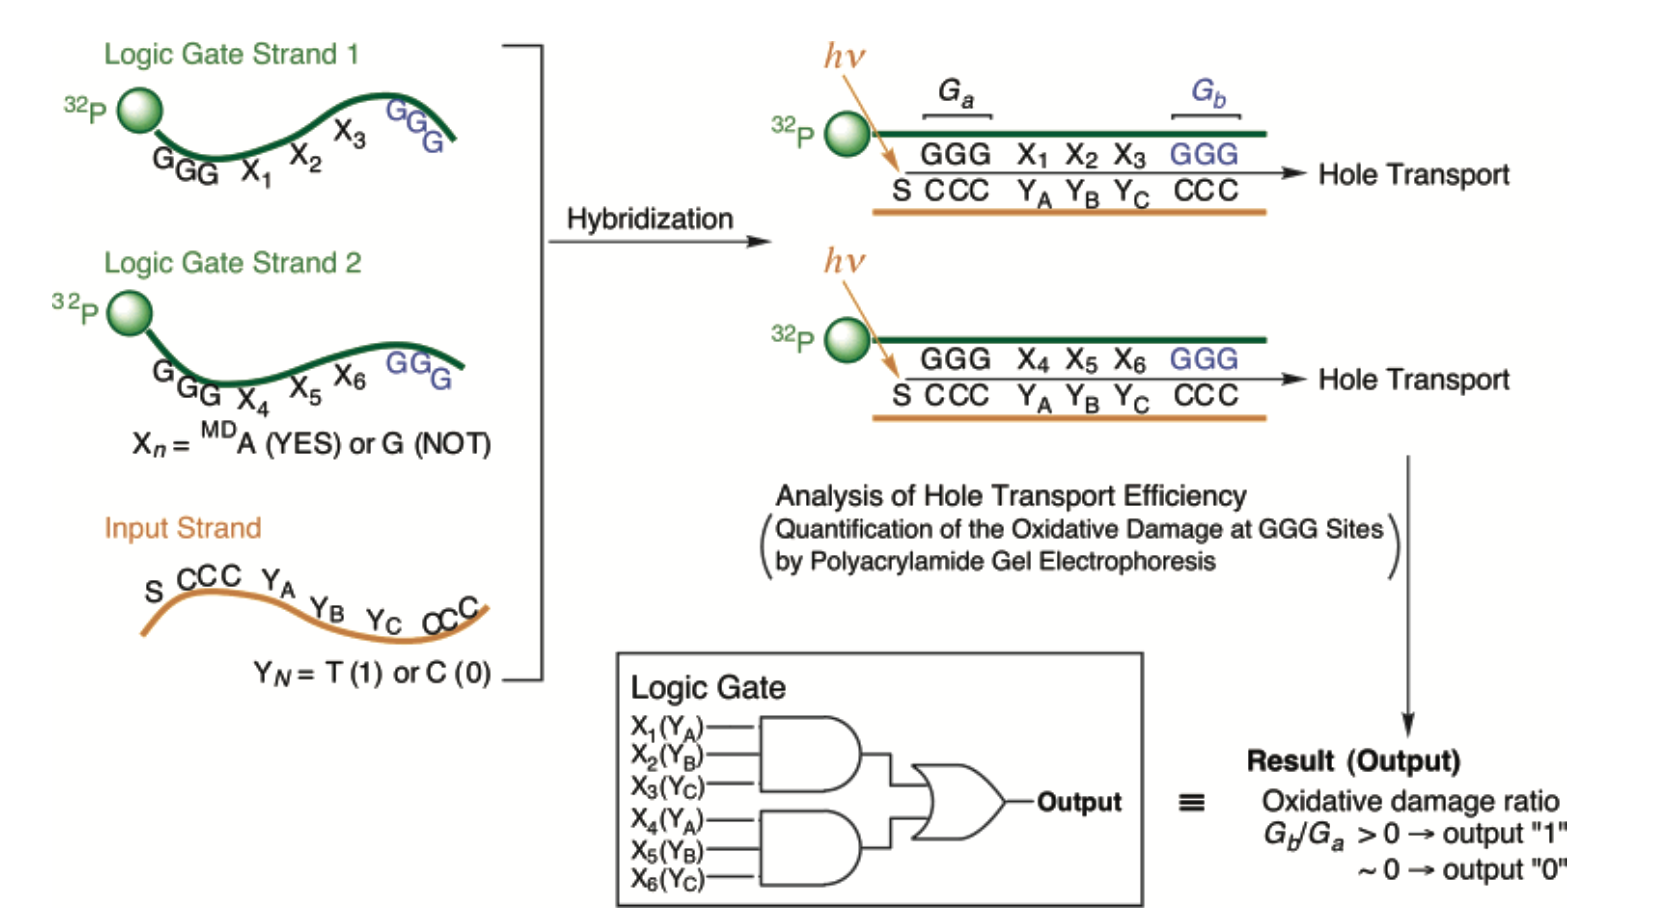
\includegraphics[width=0.95\linewidth]{images/dna-logic-gate1.png}
	\caption{DNA逻辑门的基本原理}
	\label{dna-logic-gate-implement}
\end{figure}

\newpage
在论文中,Okamoto等人用了两组实验来讲述他们的逻辑门实验,我们也把这部分放进来一并讲解。
\begin{figure}[htbp]
	\centering
	\subfigure[DNA与门实验]{
		\begin{minipage}[t]{0.47\linewidth}
			\centering
			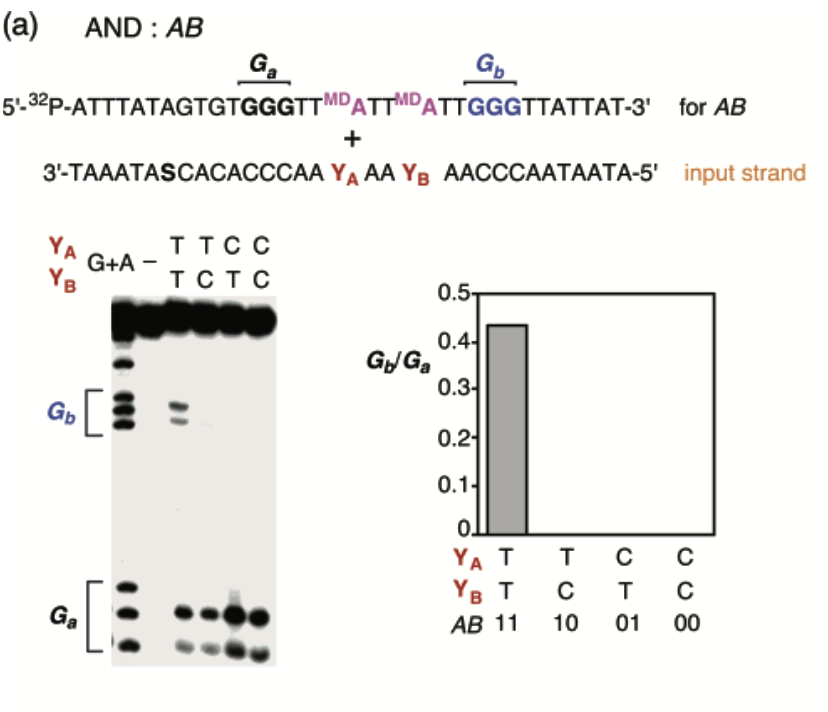
\includegraphics[width=7cm]{images/logic-gate-exper1.png}
			\label{logic-gate1}
		\end{minipage}
	}
	\subfigure[DNA或门实验]{
		\begin{minipage}[t]{0.47\linewidth}
			\centering
			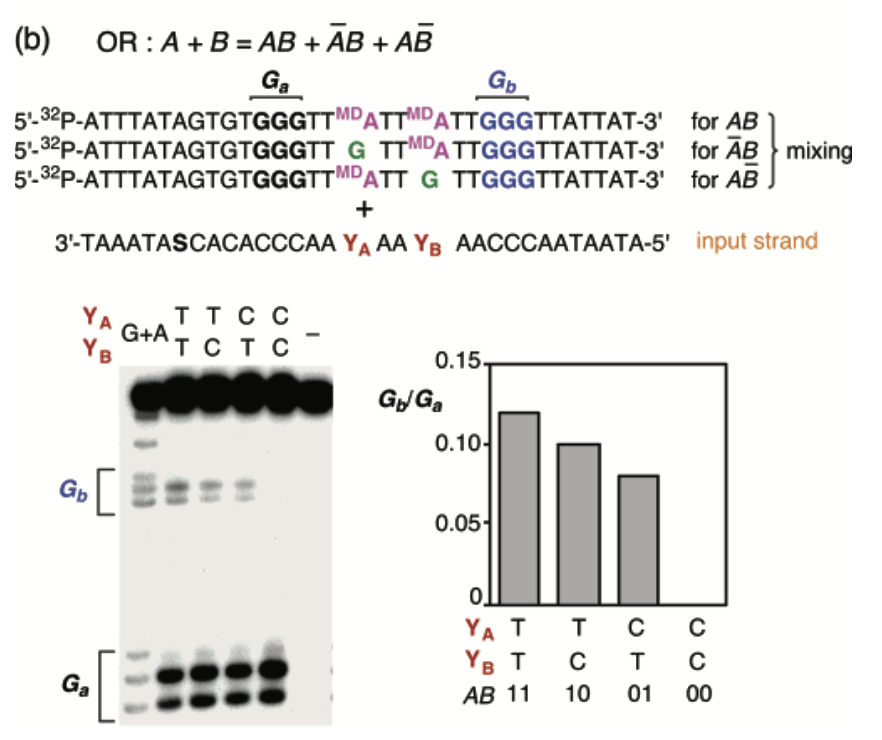
\includegraphics[width=7cm]{images/logic-gate-exper2.png}
			\label{logic-gate2}
		\end{minipage}
	}
	\caption{DNA逻辑门实验实例}
	\label{logic-gate-exper}
\end{figure}

\paragraph{DNA与门实验}在图\ref{logic-gate1}中我们可以看到逻辑门的两个输入形参都是A,即
这个逻辑门是一个只对两个T产生反应的一个与门。我们可以在图中看到左边的电泳图像。只有两个Y都是T的时候
$G_b$才会出现电泳现象。最后的$G_b \backslash G_a$也说明了这一点,只有两个输入都是1的时候才会
输出1。

\paragraph{DNA或门实验}在图\ref{logic-gate2}中我们可以看到类似上一个实验相同的结构,但是这个地方
实验者先对或运算进行了一步转换。将或运算转化成了三个合取式的析取项。所以一开始的DNA也加入了三种逻辑门,
针对11,01,10三种输入都会给出1的输出。
% 提到 Enzyme-Free Nucleic Acid Logic Circuits
% 要说到厉害之处 可以提一下这个老哥现在是在加州理工就职而且校友钱学森 in PPT
\subsection{更好的DNA逻辑门电路的实现}
在此之前人们利用各种非DNA物质对DNA逻辑门的结果进行处理,这个阶段中,人们尝试用酶,
金属离子(其中酶的影响最大),甚至一些有机物等进行逻辑电路的构建,但利用这些会对DNA结构产生破坏物质构建的DNA
逻辑电路往往在这些物质处理后就不能继续级联了,甚至连逻辑判断的功能都无法做到。

2006年,一篇“Enzyme-Free Nucleic Acid Logic Circuits”\cite{ref3}的论文被发表在science上。它提出了一种
全新的DNA逻辑门的实现形式。在文章中Erik Winfree和他的同事们提到一种叫做“Toe-hold”的反应体系(见图\ref{toe-hold-concept})。
这种方式进行计算不仅会输出双链结构,还能输出一条用于被置换下来的用于信号传递的单链。通过这种全新的反应体系,
人们可以设计出多输入的逻辑门电路,也可以通过识别反应体系中用于信号传递的单链来决定下一步的操作。

\paragraph{反应原理}
在图\ref{toe-hold-concept}中,我们可以看到左上角最大的链就是逻辑门,其中彩色的部分就是toe,
这部分可以通过DNA的合并规则与和它序列互补的分子进行合并,并且漏出一段新的toe。因此
如果我们向逻辑门中加入不同的输入,就应该会有不同的输出(图中右上角)。至此,我们通过不同的输入输出的
组合就可以让DNA完成逻辑门的操作。
\begin{figure}
	\centering
	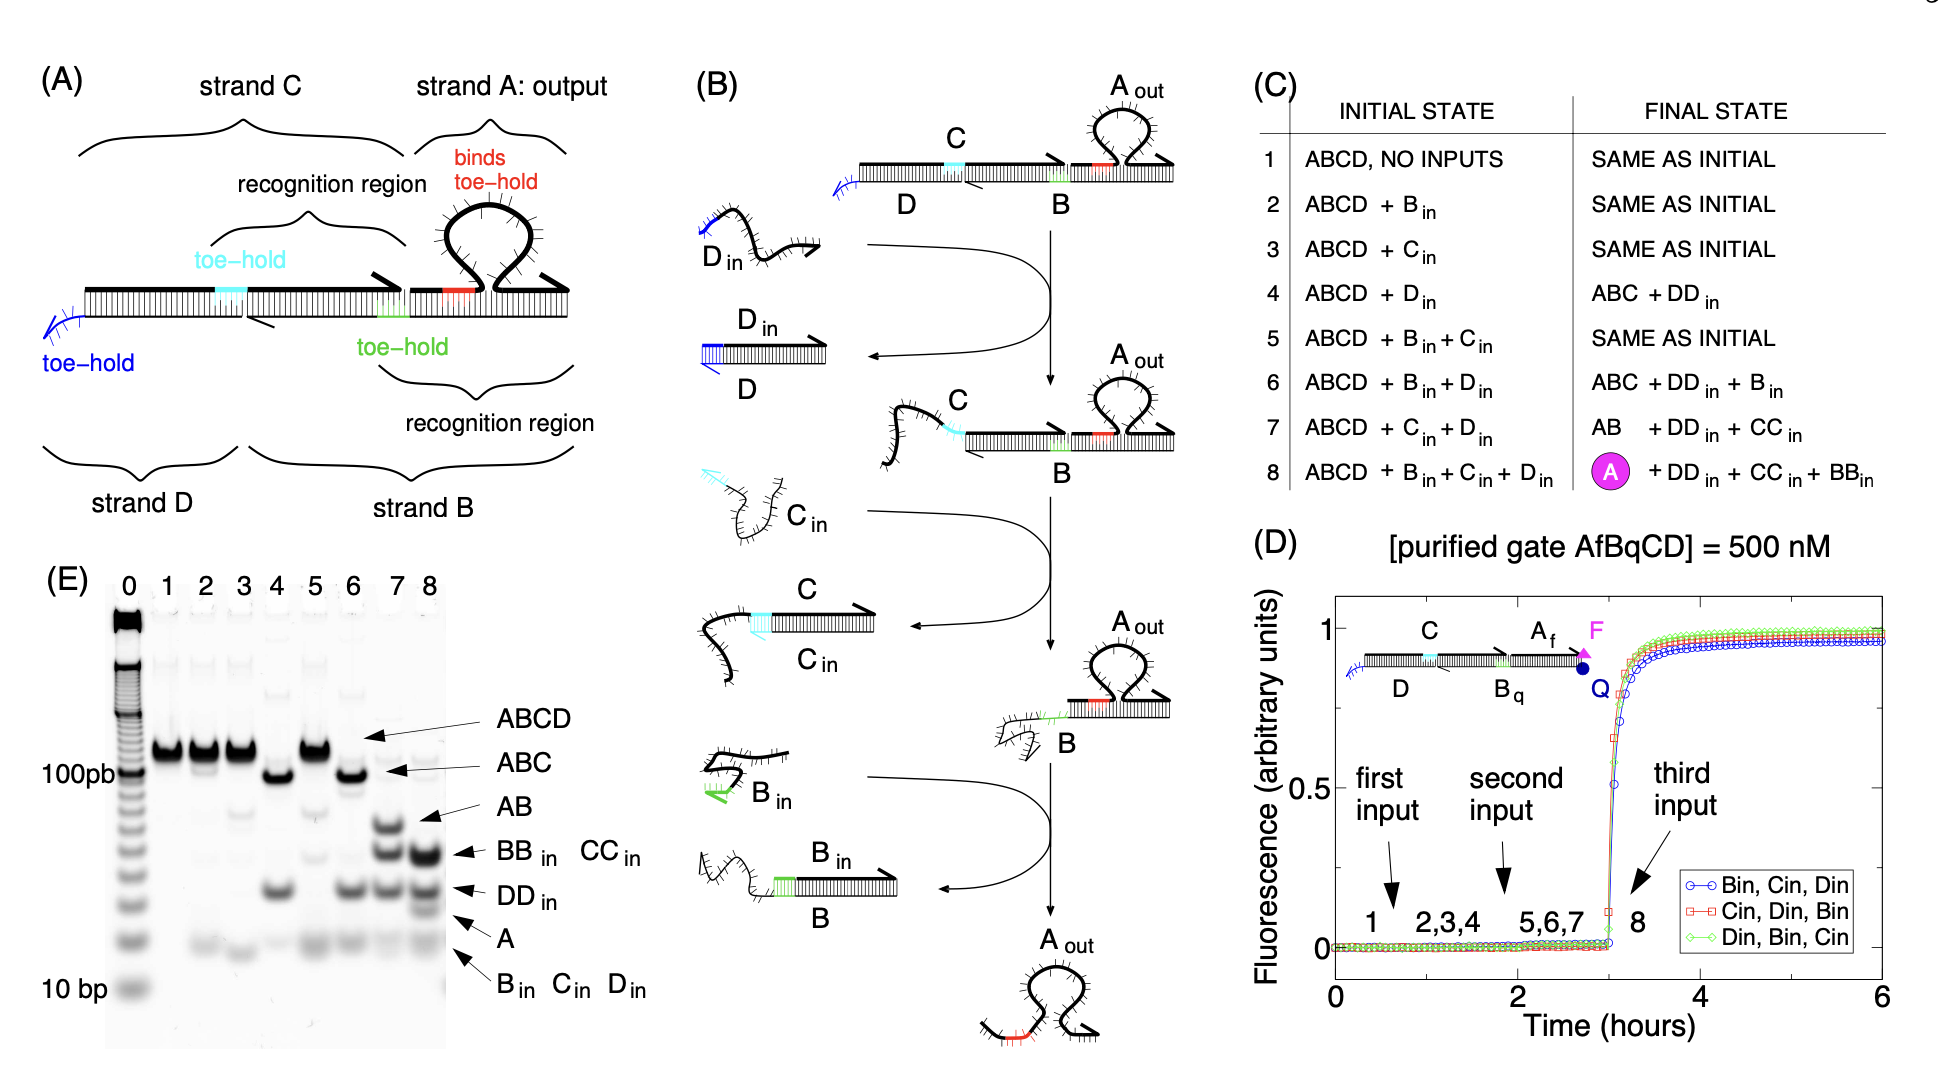
\includegraphics[width=0.9\linewidth]{images/toe-hold-concept.png}
	\caption{Toe-hold 反应体系基本原理}
	\label{toe-hold-concept}
\end{figure}
\pagebreak
\section{关于DNA计算的一些更新的应用}
\subsection{自动机}
这是来自一个关于DNA计算在自动机上面的应用\cite{ref4},作者Joanne Macdonald等人通过DNA的逻辑门实现了
一个可以下井字棋的有限自动机。在这篇论文中,巧妙地设计了与门和与非门。我们将先讲解它的门电路设计,然后讲解它的
自动机算法原理,最后我们给出它的实验结果。
\subsubsection{门电路设计}
在这篇文章中,使用了与上面不同的逻辑门电路的设计结构,但是大致思想都是相同的。即从真值表出发通过对输入输出的编解码,
来设计与之对应的DNA结构,让DNA在给定的输入上可以发出对应的、可以观测到的反应。在本实验中使用了一种环形的DNA酶。
这种DNA酶可以与一段与之匹配的DNA序列结合,然后将这段DNA序列切断。
\begin{figure}[htbp]
	\centering
	\subfigure[自动机与门和永真式]{
		\begin{minipage}[t]{0.47\linewidth}
			\centering
			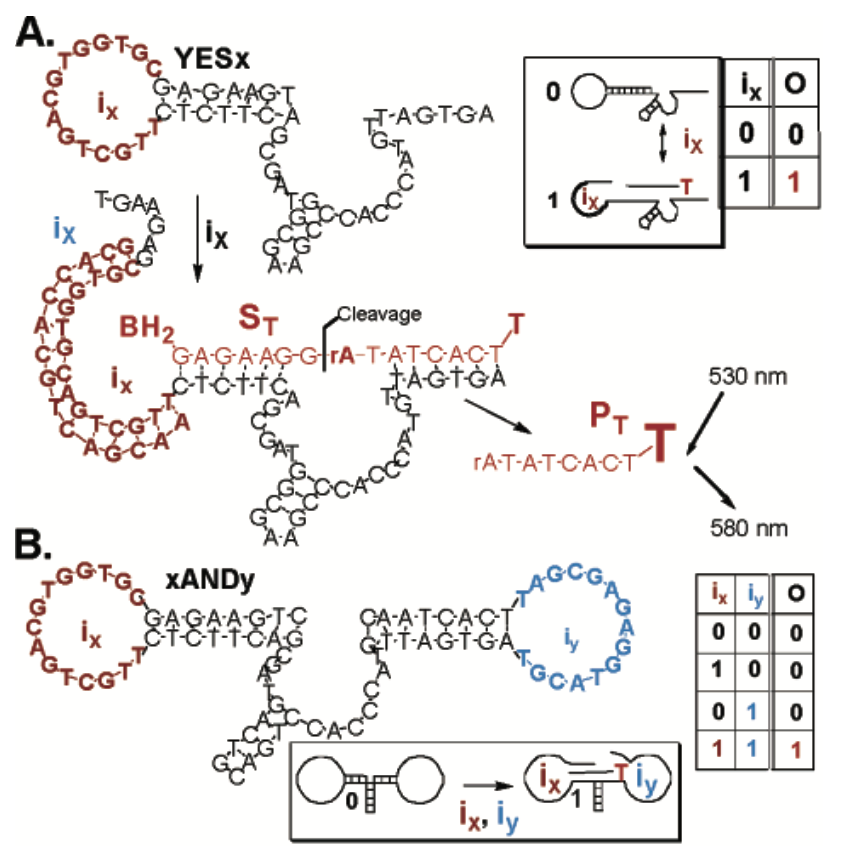
\includegraphics[width=7cm]{images/auto-machine1.png}
			\label{auto-machine1}
		\end{minipage}
	}
	\subfigure[自动机或门]{
		\begin{minipage}[t]{0.49\linewidth}
			\centering
			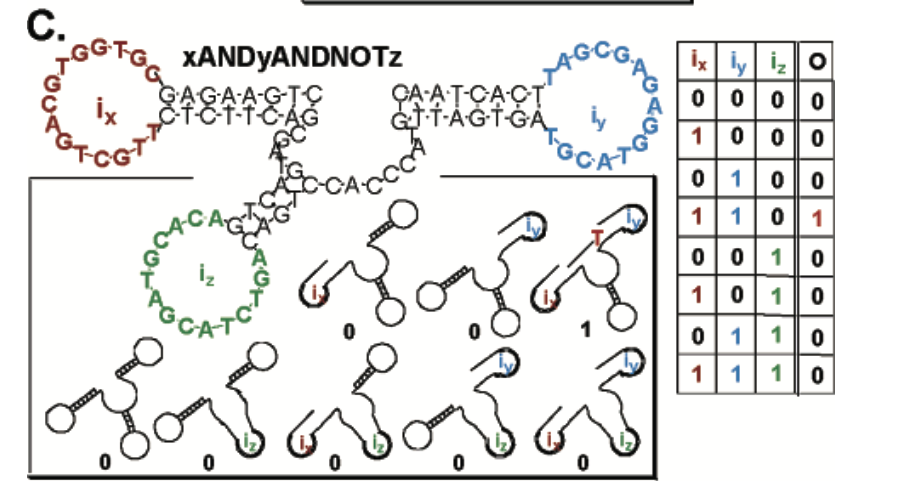
\includegraphics[width=7cm]{images/auto-machine2.png}
			\label{auto-machine2}
		\end{minipage}
	}
	\caption{自动机逻辑门电路}
	\label{auto-machine-gate}
\end{figure}

在图\ref{auto-machine1}中环形分子的两端有两个突出的序列,是用来与别的DNA序列结合的。在给定的DNA序列两端有不同的物质,有一端物质(在图中标志为\textbf{T})可以
在给定的波长下的输入的光的波长之下发出另一种波长的光;而另一端的物质(在图中标志为\textbf{BH$_2$})可以在序列完整的时候吸收\textbf{T}发出的荧光,并将其转化为热量。
这样的机制使得DNA环形分子和DNA序列分子可以相互配合来模拟逻辑门电路。我们用以与门和三输入与非门为例子来讲解门电路的具体实现。

\begin{equation}
	\centering
	f(input_k)=\left\{
	\begin{aligned}
		1 & \quad if \quad input_k \quad is \quad complementary \quad with \quad i_k \\
		0 & \quad otherwise
	\end{aligned}
	\right.
	\label{equation1}
\end{equation}

\paragraph{AND Gate}详见图\ref{auto-machine1}的下半部分B图。如果我们想要实现与门我们先拿两个
环形分子(称为$i_x$和$i_y$)与已有的环形分子的两端结合,然后这时候我们的输入可以按照下面的等式\ref{equation1}来模拟。如果我们给定的两个输入序列都是
$i_x$和$i_y$的补集,那在给定的单链DNA序列的拉伸的情况之下,环形分子的一段会与基底的DNA酶分离。在这样的充分反应之后,我们再加入一开始给定的可以发出荧光的
DNA分子序列来尝试与基底的分子的两头结合。在最后我们用仪器来检测最后有没有发出荧光,如果发出荧光,说明基底环形DNA酶已有的分子的键已经暴露并且与可以发出荧光的
DNA序列反应过了,这样一来就可以通过这种反应机理来设计一个与门。

\paragraph{Three Input AND-NOT Gate}
通过上面与门的介绍,我们可以引出一个三输入与非门来保证这个自动机可以通过多个输入来完成更加复杂的功能。在三输入与非门中\ref{auto-machine2},我们引入了
第三个环形DNA酶分子(称为$i_z$),当$i_z$的补集的DNA分子序列显现,整个大的DNA酶都会展开,从而使得DNA酶失去活性,不在起到酶的催化作用。
因此当$i_x$和$i_y$的补集分子出现,但是$i_z$的补集DNA分子没有出现的时候,整个大的分子可以显现出酶的催化作用,因此只有序列$x = y = 1; z = 0$出现的时候
整体逻辑门的输出才为1。同样的真值表也可以从图的最右侧看到。

\subsubsection{算法设计}
针对井字棋游戏,可以设计如下几条规则使得AI更加接近胜利:
\begin{enumerate}[itemsep=1.5pt,topsep=0pt,parsep=0pt]
	\item 如果下在该位置可以赢棋,那么就下在该位置
	\item 如果对手下在该位置可以赢棋,那就下在该位置
	\item 如果中心位置空闲,那么下在中心位置要优于边上和角上位置
	\item 如果角上位置空闲,那么下在角上位置要优于边上位置
	\item 如果只有边上位置空闲,那么只能下在边上位置
\end{enumerate}
因此我们就可以从上面的规则出发,将文字的规则转化为门电路的逻辑,将门电路用DNA实现一遍,最后就可以实现DNA自动机了。我们给格子从左到右、从上到下分别赋予1到9。
我们先用逻辑表达式将右上角的格子表示出来(图\ref{logic-term})。依次类推,我们可以将所有格子里面的逻辑表达式都写出来,并且将它们转化成我们已经实现好的
DNA逻辑门的形式(图\ref{logic-gate-grid})。到最后我们就可以和他展开博弈了。
\begin{figure}[htbp]
	\centering
	\subfigure[井字棋中右上格的逻辑表达式]{
		\begin{minipage}[t]{0.47\linewidth}
			\centering
			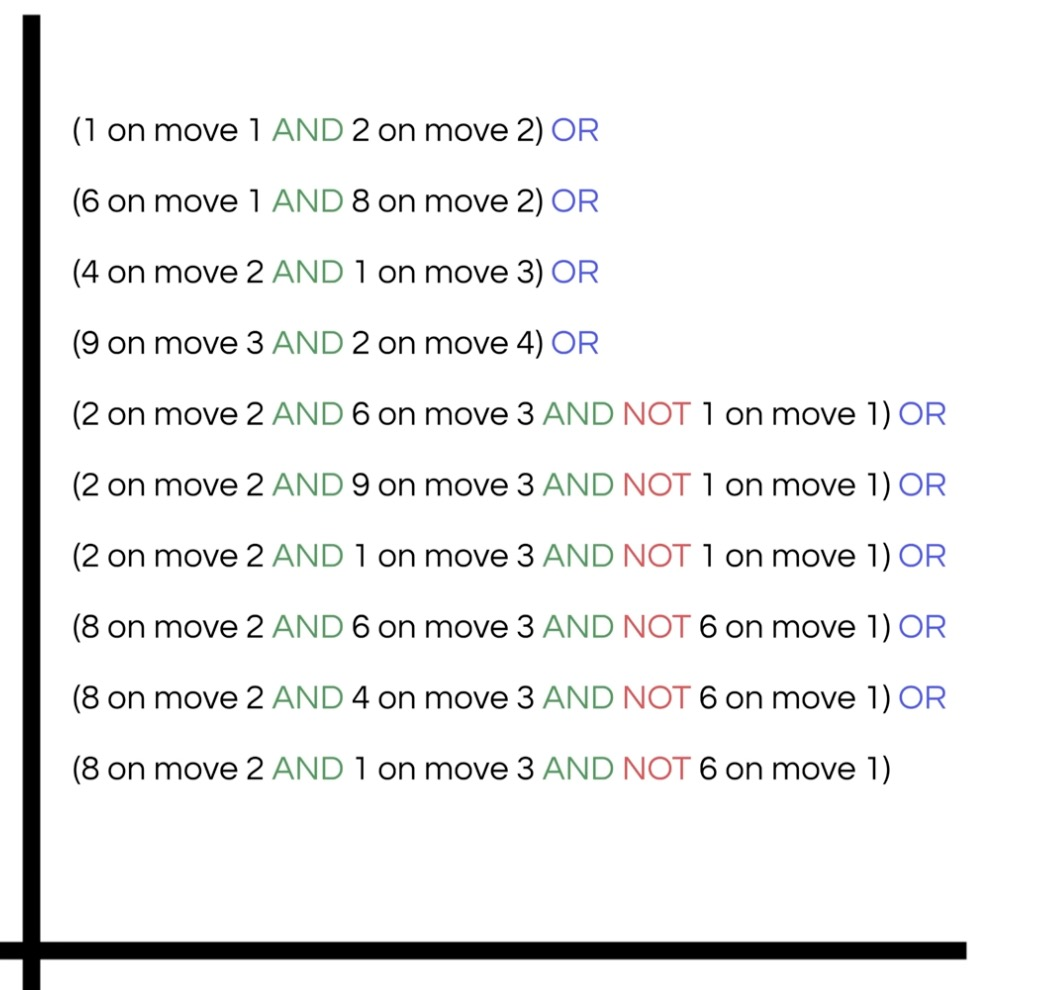
\includegraphics[width=7cm]{images/logic-term.png}
			\label{logic-term}
		\end{minipage}
	}
	\subfigure[井字棋每个格子的逻辑表达式]{
		\begin{minipage}[t]{0.49\linewidth}
			\centering
			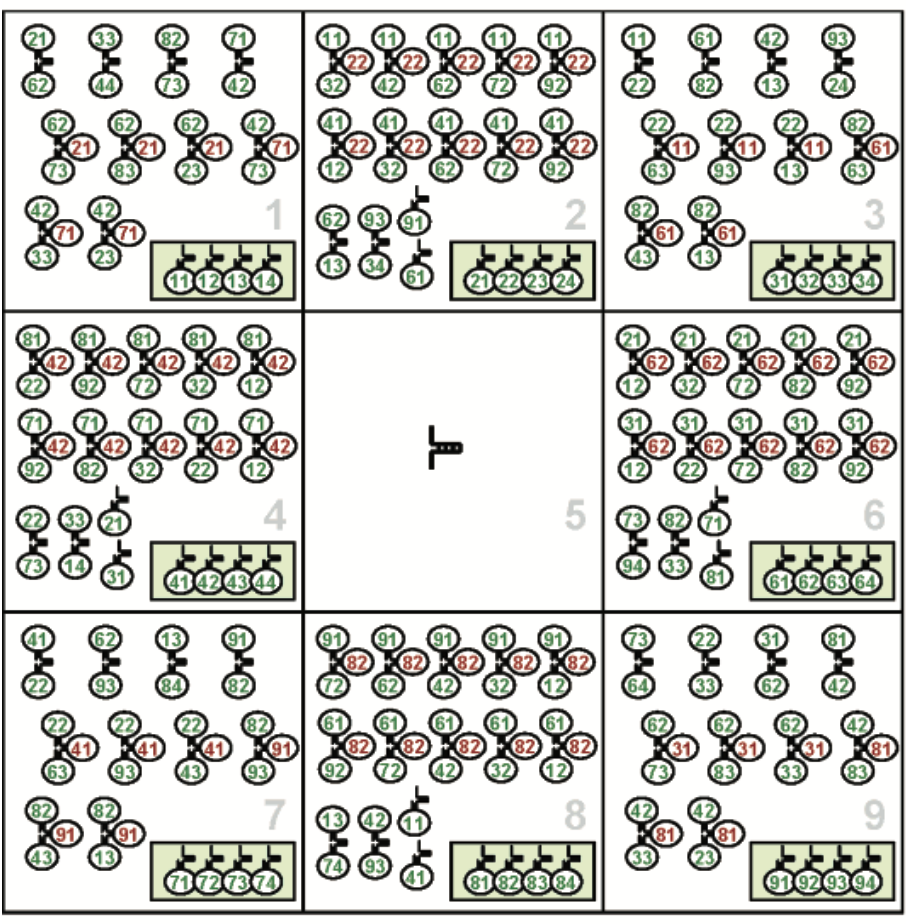
\includegraphics[width=7cm]{images/logic-gate-grid.png}
			\label{logic-gate-grid}
		\end{minipage}
	}
	\caption{自动机逻辑门电路}
\end{figure}

\subsubsection{对弈与实验结果}
在一切的准备工作准备完毕之后,就可以开始使用自动机来进行对弈,我们节选一段对弈过程来看(图\ref{automaton-battle})。
在这段节选之前,自动机先下了位置5,然后人类下了位置9,自动机给到的回应是位置2。
\begin{figure}[htbp]
	\centering
	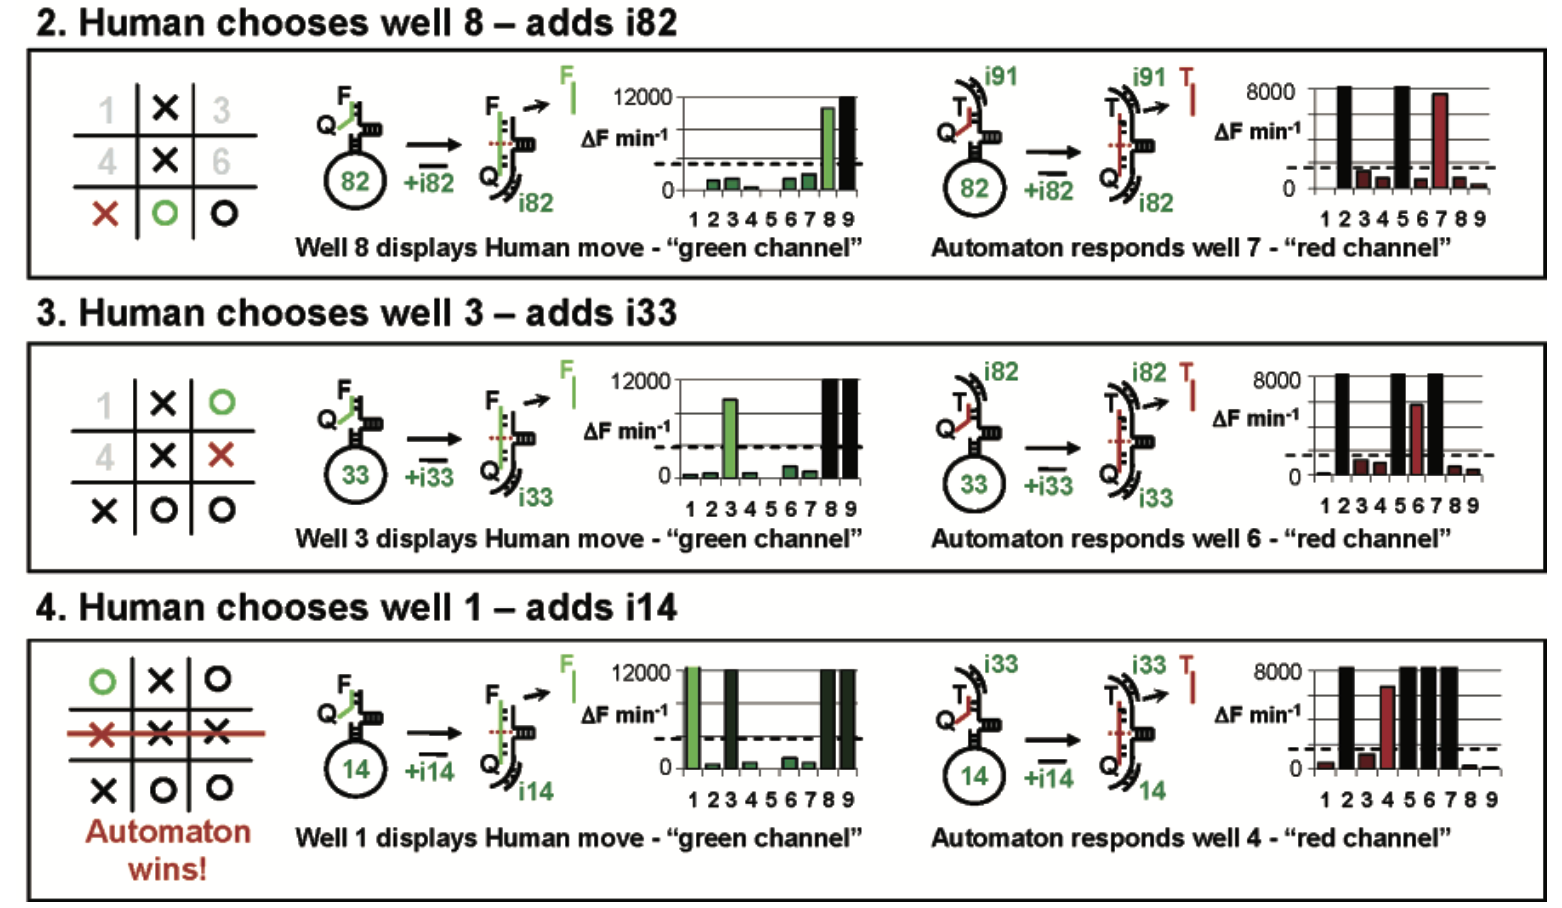
\includegraphics[width=0.95\linewidth]{images/automaton-battle.png}
	\caption{DNA自动机与人类博弈节选\protect\footnotemark[1]}
	\label{automaton-battle}
\end{figure}
\footnotetext[1]{图中的标注ixy为人类第y次行动,该次行动将棋放在位置x上}

我们以中间第三个步骤为例,在人类选择了位置3之后,即会在每一个格子对应的溶液中加入有i33的溶液
同时,i33也会与上面实现的逻辑门进行结合反应。最后加上可以发出荧光的DNA分子检测荧光,就可以看到DNA自动机
做出的回应,在这一步中,DNA自动机做出的回应是在6号位置下棋。同时在这个地方我们看到有一个特殊处理。就是如果最后荧光在别的格子中也有但是这个格子已经被占领了,
我们就默认自动机不会在这个地方做出动作。

在最后人类在1号位置下棋,然后DNA自动机在4号位置做出回应,至此我们可以验证DNA自动机在井字棋上面的能力是相当强大的。

\paragraph{一点思考}
从上面给到的实验步骤和实验结果来看,DNA自动机在串行处理的能力上确实有所欠缺。如果让硅芯片来处理
这个井字棋问题大概会用Minmax算法、alpha-beta剪枝、dfs等算法来处理这些问题。但是放到DNA自动机上面
我们必须先给出每一步可能的做法,最后再交给DNA自动机判断。同时DNA自动机需要的前期处理工作相当的繁杂。
比如我们要模拟九个格子, 每一个格子要装入对应的逻辑门的DNA序列,中间一旦出错,就会导致最后的输出错误。

但是从另一面看DNA自动机的并行计算能力是很强大的,
如果我们可以从这个中型的自动机拓展到更大型的自动机,它能处理的信息就不止是处理一个井字棋这么简单了。

\newpage
\subsection{基于DNA的神经网络实现}
这篇文章专注于用DNA来实现神经网络\cite{ref6},几位作者来自华东师范大学,基于简单的DNA门开关结构合成DNA的调控电路实现卷积神经网络算法。
采用3$\times$6大小的卷积核,可以实现超过八种模式的识别。而且这个卷积神经网络可以与另外一个DNA电路连接,构建分层网络,
这个组合网络可以识别32中模式。此外这个研究采用了一种简单的处理DNA反应的方式,可以使得计算时间从几个小时到几分钟。该方法在实现
具有复杂和噪声分类能力的高计算能力分子计算机方面具有很大的前景。

\subsubsection{结构设计}
在图\ref{dna-cnn-structure}中讲到了DNA卷积神经网络的结构以及它的反应机理。在子图a中,讲到了卷积神经网络的基本原理,简单的讲
就是卷积核在感受野上做卷积操作后讲最后的卷积结果输出为特征图像。然后再经过拉直操作,把特征图像展开为一个一维的向量,这个向量中的每一个元素的
值为输入符合该标签的概率。

在图b中,研究者讲述了如何用DNA来实现上述的卷积神经网络。在实验中我们假定输入的大小是12$\times$12的,然后我们给每一个像素点编号
分别从0-143,每一个像素点可以用一段DNA来代替,这个时候如果这个像素点是0,那么这段DNA就不会出现在DNA卷积神经网络的反应体系中;反之
则会出现在反应体系中。权重分子和输入DNA串进行结合之后就会生成新的输出,累加之后就会生成不同的$y_i$。这个地方有一个巧妙地处理
为了处理一些负值的权重,正值代表的物质和负值代表的物质是可以反应掉的。因此就从化学层面完成了减法。
\begin{figure}[htbp]
	\centering
	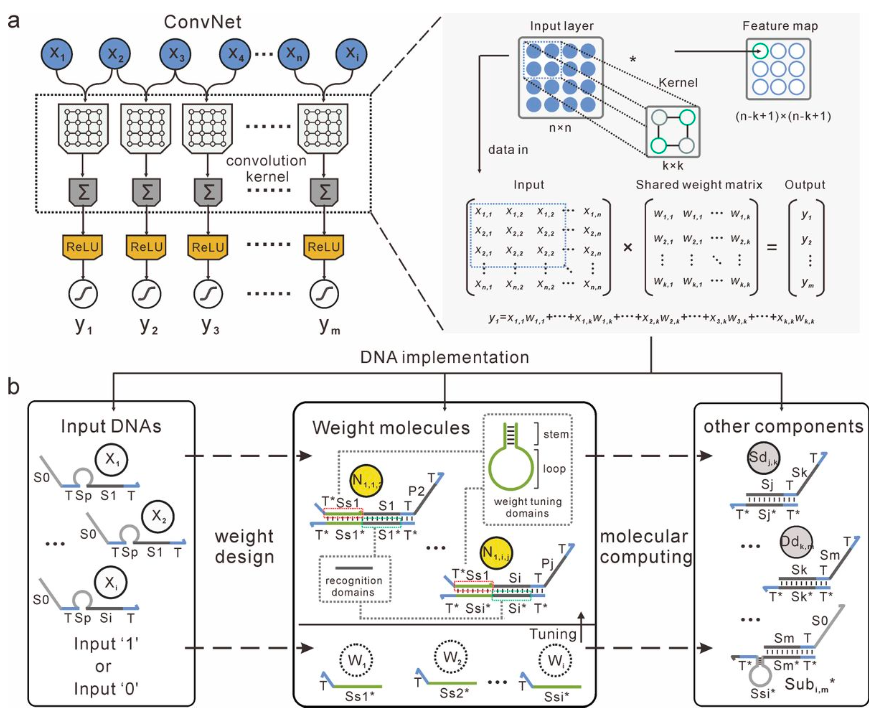
\includegraphics[width=0.8\linewidth]{images/dna-cnn-structure.png}
	\caption{DNA卷积神经网络结构}
	\label{dna-cnn-structure}
\end{figure}

\subsubsection{训练网络}
训练网络步骤见图\ref{dna-cnn-train},训练网络与我们用电子计算机来训练神经网络相同,先将目标的图片进行旋转然后映射到
12$\times$12的点阵中,点阵中的一个点就是一串DNA分子(因为只有144个像素点,没必要进行拉伸变换),然后将点阵输入进
模型进行训练,抽取特征,最后使用$argmax$函数来获得最有可能的图片匹配模式。
在这个实验中,没有用一般的参数优化方式(反向传播),而是通过调整代表权重的DNA分子在反应体系中的权重,
来调整整个卷积神经网络模型。

可以通过下面的子图e看到,这个DNA卷积神经网络在识别变换后图像的准确率方面是相当不错的。我们看到在子图e中,研究者选了两个比较相近的
的图形,Fire和Earth。我们可以通过这个图表看到,在旋转的所有角度中,DNA卷积神经网络都可以较好的识别其中模式。而且从图中也可以发现,
在绝大多数时候,分类是分的比较开的,没有分不清的情况。
\begin{figure}[htbp]
	\centering
	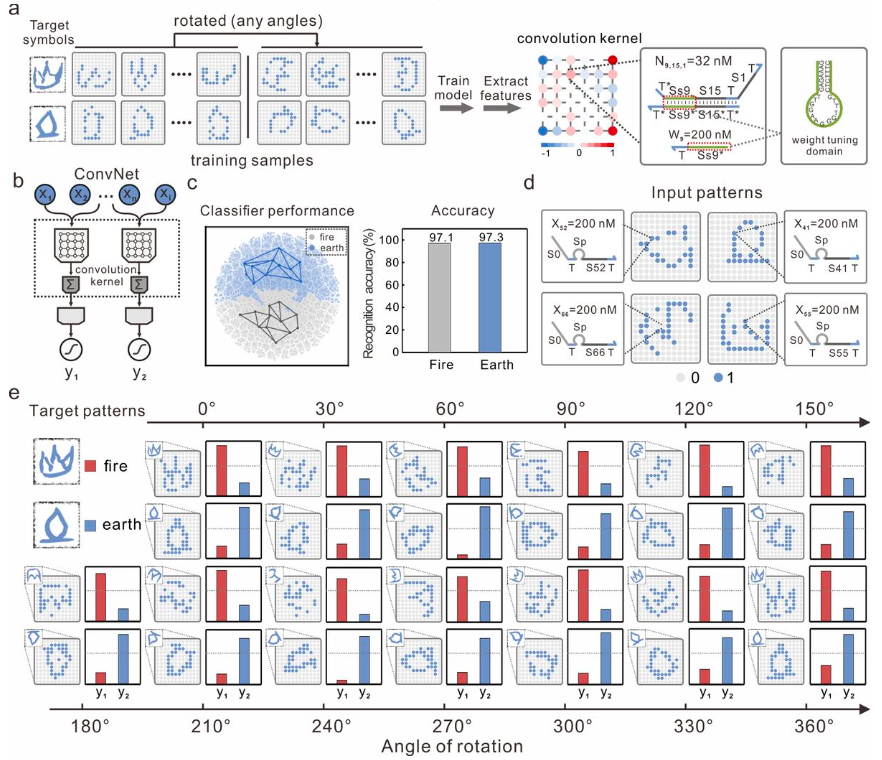
\includegraphics[width=0.8\linewidth]{images/dna-cnn-train.png}
	\caption{DNA卷积神经训练结果}
	\label{dna-cnn-train}
\end{figure}
\subsubsection{实验结果}
在后面研究者也实现了基于双重DNA电路结构的神经网络(图\ref{dna-cnn-result})。研究者在输入点阵的右上角接入了四个标记。分别标记为四类物品集合。
这个时候会先有一个DNA的分类器对这个输入点阵做分类,分类之后,可以把剩余的点阵接入到DNA卷积神经网络中去,最后根据
DNA卷积神经网络的输出,再叠加一开始的分类类别,可以做到32分类的效果。在实验结果的子图c/f中,作者用作图和枚举的方式
像我们展示了DNA神经网络的识别效果。
\newpage
\begin{figure}[htbp]
	\centering
	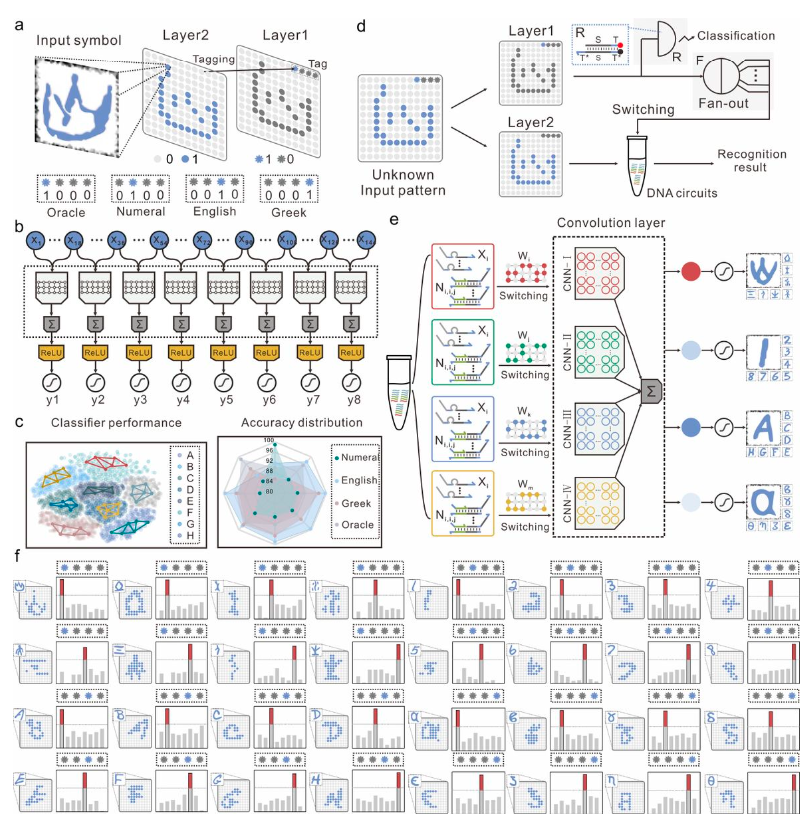
\includegraphics[width=0.9\linewidth]{images/dna-cnn-result.png}
	\caption{DNA卷积神经网络结构}
	\label{dna-cnn-result}
\end{figure}
\paragraph{一点思考}

\paragraph*{}
目前来看,用DNA来实现神经网络算是DNA计算比较前沿的研究了。作者的初衷是利用DNA计算强大并行计算方式来解决卷积问题。但是现在
应该是受制于科技水平有限,只能做出相对较为简陋的卷积神经网络模型。不过最后的识别的表现很不错,应该十分有前景。

但是另一方面,这样的DNA卷积神经网络只是在针对一个特定的问题给出答案,并没有很普遍的解决办法。如果想要想本文研究者说的一样
将这个神经网络嵌入之后的DNA计算机中,那我感觉DNA计算还要有很长的一段路要走。起码要用DNA做出有显卡那样的并行处理能力的处理结构
才能在之后的DNA计算中取得一定的成果。

\newpage
\section{讨论}
DNA计算的本质是用DNA来解决现有的数学问题。在上个世纪,Aldeman提出了用DNA分子进行计算的概念,并利用这种方法解决了一个NP完全问题——哈密顿回路问题。
这项实验证明了DNA计算的可行性,同时也为后续的DNA计算研究奠定了基础。后面也有其他研究者在考虑使用DNA计算的方法处理一些NP问题,比如尝试过用DNA计算来处理有
20个变量的3-SAT问题。但是并没有取得非常突破性的成果。之后也鲜有研究者在这个领域内深耕。不过目前已经有相关研究表明,DNA的计算能力并不能解决NP难问题。

后来DNA计算进入了一个模拟的阶段,即尝试使用DNA的结构来模拟基本的门电路。这些研究者的目的是通过模拟电子计算机中最基本的结构门电路,来让计算机完成现有计算机的一些计算。
通过设计特定的DNA序列,研究人员能够控制DNA分子之间的相互作用,并构建出具有逻辑功能的DNA电路。后来也有研究者对之前实现的DNA门电路结构做了改善,让门电路针对特定的输入做出更明显的
的反应。

在后面研究者已经开始使用前人的研究完成一些小的课题了。比如用已有的DNA门电路来模拟一个小型的有限自动机,让它可以与人们进行井字棋的对弈。
研究者的想法是这个自动机可以推广到更大型的自动机实现上,但是因为实验步骤的复杂性的限制,本文对于自动机规模的扩大提出质疑,比如我们在一个反应
体系中加入新的功能意味着要加入很多新的DNA序列溶液,这样的操作一旦出现错误,会导致自动机的功能出现致命错误。同时这样的自动机给出反应结果也是
相当慢的,在这个实验中,实验者花了几个小时才完成了一局井字棋的博弈。因此想要完美利用DNA计算的并行性完成一些大型任务,还有很多难点需要攻克。

用DNA来实现卷积神经网络是近期几位中国的研究者的成果,他们运用DNA卷积神经网络成功进行了8分类和32分类的任务。我认为这样的成果是开拓性的。
这样的模拟实验证明了DNA的并行计算能力在之后可以在更大的任务上施展。比如我们想要实现一个DNA层面的分子计算机,这样的装置肯定是必不可少的。
当然这样的研究还应该在更普适的层面上进行泛华,比如说可不可以使用DNA模拟一些类似显卡的并行计算的处理单元。我相信如果这些研究可以做出成果,
人类对于DNA计算的梦想离实现也就不远了。
% citation 
\newpage
\begin{thebibliography}{10}
	\bibitem{ref1} L. M. Adleman, "Molecular computation of solutions to combinatorial problems," Science, vol. 266, no. 5187, pp. 1021-1024, Nov. 1994, doi: 10.1126/science.7973651.
	\bibitem{20v}  R. S. Braich, N. Chelyapov, C. Johnson, P. W. Rothemund, and L. Adleman, “Solution of a 20-variable 3-SAT problem on a DNA computer,” Science, vol. 296, no. 5567, pp. 499–502, 2002.
	\bibitem{ref2} A. Okamoto, K. Tanaka, and I. Saito, “DNA logic gates,” Journal of the American Chemical Society, vol. 126, no. 30, pp. 9458–9463, 2004.
	\bibitem{ref3} G. Seelig, D. Soloveichik, D. Y. Zhang, and E. Winfree, “Enzyme-free nucleic acid logic circuits,” Science, vol. 314, no. 5805, pp. 1585–1588, 2006.
	\bibitem{ref4} J. Macdonald, Y. Li, M. Sutovic, H. Lederman, K. Pendri, W. Lu, B. L. Andrews, D. Stefanovic, and M. N. Stojanovic, “Medium scale integration of molecular logic gates in an automaton,” Nano Letters, vol. 6, no. 11, pp. 2598–2603, 2006.
	\bibitem{ref6} X. Xiong et al., “Molecular convolutional neural networks with DNA regulatory circuits,” Nature Machine Intelligence, vol. 4, no. 7, pp. 625–635, 2022. doi:10.1038/s42256-022-00502-7
\end{thebibliography}
\end{document}